\documentclass[tikz,border=2pt,11pt]{standalone}
\usetikzlibrary{arrows.meta}
\usetikzlibrary{positioning}
\usepackage{amsmath}
\usepackage{amssymb}
\usepackage{tikz}
\newcommand{\C}{\mathbb C}
\newcommand{\R}{\mathbb R}
\newcommand{\Z}{\mathbb Z}
\newcommand{\N}{\mathbb N}
\DeclareMathOperator{\HS}{HS}
\DeclareMathOperator{\HH}{HH}
\DeclareMathOperator{\tr}{tr}
\DeclareMathOperator{\supp}{supp}
\DeclareMathOperator{\con}{con}
\DeclareMathOperator{\id}{id}
\begin{document}
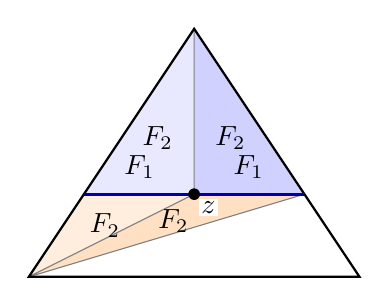
\begin{tikzpicture}[scale=1.05]
 \coordinate (A) at (-2,0);
 \coordinate (B) at (2,0);
 \coordinate (C) at (0,3);
 \coordinate (L) at (-1.3333,1);
 \coordinate (R) at (1.3333,1);
 \coordinate (z) at (0,1);
 \fill[blue!9] (L)--(z)--(C)--cycle;
 \fill[blue!18] (z)--(R)--(C)--cycle;
 \fill[orange!13] (L)--(z)--(A)--cycle;
 \fill[orange!24] (z)--(R)--(A)--cycle;
 \draw[thin,gray] (z)--(A) (A)--(R) (z)--(C);
 \draw[thick] (A)--(B)--(C)--cycle;
 \draw[very thick,blue!65!black] (L)--(R);
 \fill (z) circle (2pt) node[below right=2pt,fill=white,inner sep=1pt] {$z$};
 \node at (-0.44,1.68) {$F_2$};
 \node at (0.44,1.68) {$F_2$};
 \node at (-1.08,0.62) {$F_2$};
 \node at (-0.25,0.67) {$F_2$};
 \node[above=2pt] at (-0.66,1) {$F_1$};
 \node[above=2pt] at (0.66,1) {$F_1$};
\end{tikzpicture}
\end{document}
